\begin{figure}[H]
\centering
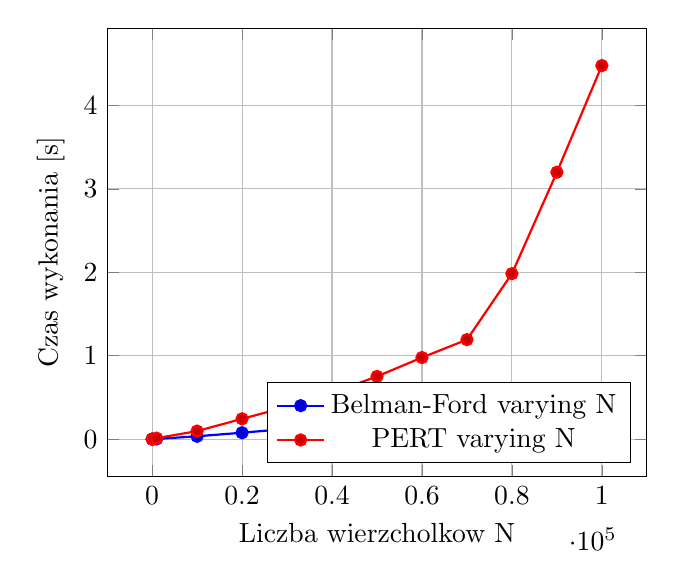
\begin{tikzpicture}
\begin{axis}[
xlabel = {Liczba wierzcholkow N},
ylabel = {Czas wykonania [s]},
legend pos = south east,
grid = both,
]
\addplot + [mark = *, thick] coordinates
    {
(10, 0.0)(100, 0.0009999275207519531)(1000, 0.003000497817993164)(10000, 0.0348203182220459)(20000, 0.07751870155334473)(30000, 0.12386822700500488)(40000, 0.1819767951965332)(50000, 0.22945022583007812)(60000, 0.2892603874206543)(70000, 0.3352177143096924)(80000, 0.4021949768066406)(90000, 0.4607203006744385)(100000, 0.5247666835784912)};
\addlegendentry
{Belman-Ford varying N}
\addplot + [mark = *, thick] coordinates
    {
(10, 0.0)(100, 0.001001119613647461)(1000, 0.012100934982299805)(10000, 0.0970010757446289)(20000, 0.24403619766235352)(30000, 0.3881571292877197)(40000, 0.5543763637542725)(50000, 0.7522757053375244)(60000, 0.9783093929290771)(70000, 1.1930625438690186)(80000, 1.9836766719818115)(90000, 3.199394464492798)(100000, 4.477366209030151)};
\addlegendentry
{PERT varying N}
\end{axis}
\end{tikzpicture}
\caption
{Por�wnanie czas�w wykonania algorytm�w Belman-Ford i PERT}
\label{fig:time_measurements}
\end{figure}
